\documentclass[10pt]{beamer}
\usetheme{AAUsimple}

\usepackage[utf8]{inputenc}
\usepackage[T1]{fontenc}
\usepackage[danish]{babel}
\usepackage{helvet}
\usepackage{listings}

\newcommand{\chref}[2]{%
  \href{#1}{{\usebeamercolor[bg]{AAUsimple}#2}}%
}


\author{}
\institute{
  Institut for Matematiske Fag\\
  Aalborg Universitet\\
  Danmark

}
\pgfdeclareimage[height=1.5cm]{titlepagelogo}{AAUgraphics/aau_logo_new}
\titlegraphic{\pgfuseimage{titlepagelogo}}


\title{Projekt Strukturering}
\subtitle{Workshop 2}
\date{5. september 2019}

\begin{document}

% Title page
{\aauwavesbg
  \begin{frame}[plain,noframenumbering]
  \titlepage
\end{frame}}

% Table of contents
\begin{frame}{Agenda}{}
\tableofcontents
\end{frame}

% Main content

\section{Opdeling af Projektfiler}

\begin{frame}[containsverbatim]{Opdeling Projektfiler}{Mappestruktur}
  \begin{columns}
    \begin{column}{0.5\textwidth}
      \begin{tikzpicture}
        \draw[color=black!60!white]
        \FTdir(\FTroot,root,P1){
          \FTfile(root,master.tex)
          \FTfile(root,master.pdf)
          \FTdir(root,incl,incl){
            \FTdir(incl,main,main) {
              \FTfile(main,graph\_theory.tex)
            }
            \FTdir(incl,misc,misc) {
              \FTfile(misc,preface.tex)
              \FTfile(misc,introduction.tex)
            }
            \FTdir(incl,app,app) {
              \FTfile(app,notation.tex)
            }
          }
          \FTdir(root,fig,fig) {
            \FTdir(fig,img,img){
              \FTfile(img,digraph.pdf)
            }
            \FTdir(fig,tab,tab) {
              \FTfile(tab,summary\_table.tex)
            }
          }
        };
      \end{tikzpicture}
    \end{column}
    \begin{column}{0.5\textwidth}
      \begin{block}{}
        Eksempel på dele af en mappestruktur for et P1-projekt.
      \end{block}
      \begin{block}{}
        Forskellige typer af indhold ligger i forskellige undermapper.
      \end{block}
    \end{column}
  \end{columns}
\end{frame}

\begin{frame}[containsverbatim]{Opdeling af Projektfiler}{Inkluder Filer i Masteren}
  \begin{block}{master.tex}
\begin{verbatim}
  \documentclass[10pt]{report}
  \begin{document}
  \include{incl/misc/preface}
  \include{incl/misc/introduction}
  \include{incl/main/graph_theory}
  \appendix
  \include{incl/app/notation}
  \end{document}
\end{verbatim}
  \end{block}

  \begin{block}{graph\_theory.tex}
\begin{verbatim}
\chapter{Grafteori}
Dette kapitel omhandler...
\input{fig/tab/summary_table.tex}
\end{verbatim}
  \end{block}
\end{frame}

\begin{frame}[containsverbatim]{Opdeling af Projektfiler}{Preamble}
  \begin{block}{preamble.tex}
\begin{verbatim}
\usepackage[utf8]{inputenc}           % DK bogstaver ind
\usepackage[T1]{fontenc}              % DK bogstaver ud
\usepackage[danish]{babel}            % DK formattering
\usepackage{mathtools,amssymb}        % Matematik
\usepackage{graphicx}                 % Billedfil-support
\end{verbatim}
  \end{block}
    \begin{block}{master.tex}
\begin{verbatim}
\documentclass[10pt]{report}
\usetheme{AAUsimple}

\usepackage[utf8]{inputenc}
\usepackage[T1]{fontenc}
\usepackage[danish]{babel}
\usepackage{helvet}
\usepackage{listings}

\newcommand{\chref}[2]{%
  \href{#1}{{\usebeamercolor[bg]{AAUsimple}#2}}%
}


\author{}
\institute{
  Institut for Matematiske Fag\\
  Aalborg Universitet\\
  Danmark

}
\pgfdeclareimage[height=1.5cm]{titlepagelogo}{AAUgraphics/aau_logo_new}
\titlegraphic{\pgfuseimage{titlepagelogo}}

\begin{document}
...
\end{document}
\end{verbatim}
  \end{block}
\end{frame}

\section{Fejlmeddelelser}

\begin{frame}[containsverbatim]{Fejlmeddelelser}{Typer}
  \begin{itemize}
  \item \LaTeX\ giver fejl hvis en kommando er skrevet forkert
  \item Det sker \textbf{hele tiden for os alle}
  \item Man skal derfor vide, hvordan man retter fejl
  \item En fejlmeddelelse starter altid med et udråbstegn
  \item Editors som TeXMaker samler fejlmeddelelser fra log-filen
  \item Brug Google - andre har helt sikkert haft den samme fejl
  \end{itemize}

\begin{verbatim}
! Too many }'s.
l.6 \frac 1}{2}

! Undefined control sequence.
l.6 \dtae

! Missing $ inserted
\end{verbatim}
\end{frame}

\begin{frame}[containsverbatim]{Fejlmeddelelser}{Strategi}
  \begin{itemize}
  \item Mange fejl kan fanges ved at kompilere ofte
  \item Nogle gange ved man ikke, hvor i dokumentet fejlen er
  \item Brug evt. udelukkelsesmetoden her---udkommenter indtil det virker igen, så ved du, at fejlen er i den udkommenterede del af koden
  \end{itemize}
\end{frame}

\section{Floats og Andre Blokmiljøer}

\begin{frame}{Floats og Andre Blokmiljøer}{Floats}

  \begin{block}{Floats}
    \begin{itemize}
  \item Floats bruges til indhold som ikke må brydes over flere sider
  \item De kan indeholde captions til at beskrive indholdet
  \item En caption \textbf{SKAL} kunne forklare indholdet uden man behøver læse brødteksten
  \item De er nummererede og man kan henvise til dem i brødteksten
  \end{itemize}
  \end{block}

  \begin{block}{Typiske Floats}
    \begin{itemize}
    \item Figurer
    \item Tabeller
    \end{itemize}
  \end{block}
\end{frame}

\begin{frame}[containsverbatim]{Floats og Andre Blokmiljøer}{Figurer}
  \begin{columns}
    \begin{column}{0.6\textwidth}
\begin{verbatim}
\begin{figure}[htbp]
  \centering
  \includegraphics{fig/img/taylor.pdf}
  \caption{Taylor approksimation
    af $f(x) = \log(x)$.}
  \label{fig:taylor}
\end{figure}
\end{verbatim}
    \end{column}
    \begin{column}{0.4\textwidth}
      \begin{figure}[h]
        \centering
        \includegraphics[width=\linewidth]{img/taylor.pdf}
        \caption{Taylor approksimation af $f(x) = \log(x)$.}
        \label{fig:taylor}
      \end{figure}
    \end{column}
  \end{columns}
\end{frame}


\begin{frame}[containsverbatim]{Floats og Andre Blokmiljøer}{Tabeller}
\begin{columns}
  \begin{column}{0.6\textwidth}
    \begin{verbatim}
\begin{table}[htbp]
 \begin{center}
   \begin{tabular}{c|c|c}
    $n$ & $f^{(n)}(x)$ & $f^{(n)}(0)$\\
    \hline
    1 & $\log(x)$        &  0 \\
    2 & $\frac{1}{x}$    &  1 \\
    3 & $-\frac{1}{x^2}$ & -1 \\
    \hline
   \end{tabular}
 \end{center}
 \caption{Taylor}
 \label{tab:taylor_lnx}
\end{table}
\end{verbatim}
  \end{column}
  \begin{column}{0.4\textwidth}
  \begin{table}[h]
  \begin{center}
    \begin{tabular}{c|c|c}
     $n$ & $f^{(n)}(x)$     & $f^{(n)}(0)$\\\hline
     1   & $\log(x)$        & 0           \\
     2   & $\frac{1}{x}$    & 1           \\
     3   & $-\frac{1}{x^2}$ & -1          \\
      \hline
    \end{tabular}
  \end{center}
  \caption{Evaluering af $f$ og de afledte i $a=1$.}
  \label{tab:taylor_lnx}
\end{table}
\end{column}
\end{columns}
\end{frame}


\begin{frame}[containsverbatim]{Floats og Andre Blokmiljøer}{Andre Blokmiljøer}
  \begin{columns}
    \begin{column}{0.6\textwidth}
      \begin{block}{Ikke-ordnede lister}
\begin{verbatim}
\begin{itemize}
\item $\alpha$
\item $\beta$
\item $\zeta$
\end{itemize}
\end{verbatim}
      \end{block}
      \begin{block}{Ordnede lister}
\begin{verbatim}
\begin{enumerate}
\item $\delta$
\item $\epsilon$
\item $\phi$
\end{enumerate}
\end{verbatim}
      \end{block}
    \end{column}
    \begin{column}{0.4\textwidth}
      \begin{block}{}
        \begin{itemize}
        \item $\alpha$
        \item $\beta$
        \item $\zeta$
        \end{itemize}
      \end{block}
      \begin{block}{}
        \begin{enumerate}
        \item $\delta$
        \item $\epsilon$
        \item $\phi$
        \end{enumerate}
      \end{block}
    \end{column}
  \end{columns}
\end{frame}

\begin{frame}[containsverbatim]{Floats og Andre Blokmiljøer}{Krydsreferencer}
  \begin{columns}
    \begin{column}{0.6\textwidth}
\begin{verbatim}
\section{Krydsreferencer}
\label{krydsrefs}

Se Tabel \ref{tab:taylor_lnx}
og Figur \ref{fig:taylor}.

Betragt følgende:
\begin{equation}
  \label{eq:1}
  \sum_{k=0}^{n} k =
    \frac{n(n+1)^2}{2} .
\end{equation}

Gauss opdagede \eqref{eq:1}
i 1800-tallet.
\end{verbatim}
    \end{column}
    \begin{column}{0.4\textwidth}
      Se Tabel \ref{tab:taylor_lnx}
      og Figur \ref{fig:taylor}.

      Betragt følgende:
      \begin{equation} \label{eq:1}
        \sum_{k=0}^{n} k = \frac{n(n+1)^2}{2} .
      \end{equation}

      Gauss opdagede \eqref{eq:1}
      i 1800-tallet.
    \end{column}
  \end{columns}
\end{frame}


\section{Opgaver}

\begin{frame}[containsverbatim]{Opgaver}{Opgave 1}
  \begin{columns}
    \begin{column}{0.5\textwidth}
      Lav et \LaTeX-dokument, hvori I opskriver en Taylor-udvikling for \(e^{x}\), inkluderer et billede som figur, og opskriver en tabel over værdier for \(n = 1, 2, 3\).
      \begin{itemize}
      \item Lav en undermappe i mappen for dette kursus med strukturen vist til højre:
      \item Hent \texttt{fig/img/taylor.pdf}\footnotemark[1]
      \item Udfyld de tre \texttt{.tex} filer med relevant indhold
      \end{itemize}
    \end{column}
    \begin{column}{0.5\textwidth}
      \begin{tikzpicture}
        \draw[color=black!60!white]
        \FTdir(\FTroot,root,opgave){
          \FTfile(root,master.tex)
          \FTfile(root,master.pdf)
          \FTdir(root,incl,incl){
            \FTdir(incl,main,main) {
              \FTfile(main,taylor.tex)
            }
          }
          \FTdir(root,fig,fig) {
            \FTdir(fig,img,img) {
              \FTfile(img,taylor.pdf)
            }
            \FTdir(fig,tab,tab) {
              \FTfile(tab,taylor\_vals.tex)
            }
          }
        };
      \end{tikzpicture}
    \end{column}
  \end{columns}
  \footnotetext[1]{Hvorhenne kan de hente denne fil?}
\end{frame}

\end{document}

%%% Local Variables:
%%% mode: latex
%%% TeX-master: t
%%% End:
